\documentclass[a4paper,12pt]{article}
\usepackage{listings}

%% Language and font encoding
\usepackage[english]{babel}
\usepackage[utf8x]{inputenc}
\usepackage[T1]{fontenc}

%% Sets page size and margins
\usepackage[a4paper,top=3cm,bottom=2cm,left=3cm,right=3cm,marginparwidth=1.75cm]{geometry}

%% Useful packages
\usepackage{amsmath}
\usepackage{graphicx}
\usepackage[colorinlistoftodos]{todonotes}
\usepackage[colorlinks=true, allcolors=blue]{hyperref}
\usepackage{ragged2e}


\begin{document}
\begin{titlepage}
\begin{center}
		{\Large \textbf{Ludwig-Maximilians-Universität München}} \\
	\vspace{35mm}
{\bfseries\LARGE{Criminal recidivism after prison and electronic monitoring}} \\{\bfseries\large{by Rafael Di Tella and Ernesto Schargrodsky}} 
			\vspace{10mm}\\
            {\Large Causal Inference for Policy Evaluation } \\
			\vspace{2mm}
            {\Large{Bakai Baiazbekov
		\renewcommand\thefootnote{*}\footnote{B.Baiazbekov@campus.lmu.de}}}\\
        {\today}	\\
		\vspace{8mm}
		\begin{figure}[h] 
        \begin{center}

\includegraphics[width=0.6\textwidth]{lmu_siegel.png} \
\end{center}
\end{figure}%
	\end{center}

\end{titlepage}


\pagenumbering{Roman}
\setcounter{page}{2}
\tableofcontents  
\newpage

\pagenumbering{arabic}
\setcounter{page}{1}


\section{Introduction}

All societies must decide what to do with those who commit crimes. While a standard approach for centuries has been to incarcerate offenders but since the technology doesn't stay at same place, recently was proposed to use electronic monitoring bracelets for offenders to monitor them remotely. Electronic monitoring of offenders has been in use for just over two decades and motives for using it remain diverse. Some agencies that use EM attempt to deliver humane and affordable sanctions while others seek to relieve jail crowding or to avoid the construction of new jails. 
As the fiscal burden of the prison population has increased and as the electronic monitoring technology became cheaper and safer with more precise, where these devices can track GPS, recognize voice with machine learning techniques and measure the trans-dermal measurement of alcohol or drug consumption. In the history, there was prisons called "panopticon", where inmates could be watched continually by guards who could not be seen.  

In this paper authors studied electronic monitoring in the Province of Buenos Aires, Argentina. They measured recidivism through rearrest rates of offenders treated with electronic monitoring since the programs inception in the late 1990s. As a benchmark, they took a sample of former prisoners of similar observable characteristics treated with incarceration, where they found a large negative and statistically significant correlation between electronic monitoring and rearrest rates.   

This paper based on measurement of causal effect of criminal recidivism rate in the city of Buenos Aires. By focusing on the rearrest rates of two groups: individuals released from prison and individuals released from electronic monitoring program. Detainees are randomly assigned to different types of judges, where ideological di

fferences across judges translate into large differences in the allocation of electronic monitoring. Taking into account this type of characteristics of judges, authors argue that there is a large, negative effect on criminal recidivism of treating individuals with electronic monitoring relative to prison. 

Every year a large number of individuals are sent to prison in Argentina. By 2007, the Penitentiary Service of the Buenos Aires hosted of approximately 26,990 inmates which represented 44.5 percent of the total population under penal supervision of the whole country. The conditions of confinement are extremely poor, perhaps because the inmate population held in prisons and jails experienced a large increase from 12,223 in 1994 to 30,721 in 2005, with increase 18,498 in 11 years and without a corresponding increase in infrastructure investment. Given that prisons are costly to build and run and often involve cruel treatment of fellow citizens, possibly contributing to the conversion of inmates into "hardened" criminals, it is unsurprising that alternatives to imprisonment have been tried out. One of the more intriguing experiments in this area is the substitution of electronic monitoring for incarceration. If we look to statistics, by 2010, more than 500,000 people in the United States and Europe alone had been treated with electronic monitoring, in spite of the obvious complexity of a full cost-benefit analysis. In this paper, authors tried to contribute to an evaluation of electronic monitoring by providing the evidence on one of the estimates needed for such exercise: the difference between the recidivism rate of offenders treated with electronic monitoring and the recidivism rate of offenders released from a standard prison. 

Electronic monitoring arises several debates such as that spending time under electronic monitoring rather than incarceration might make low punishment salient, implying a positive relationship between light punishment, electronic monitoring, and recidivism. On the other hand, some find a negative relationship, for instance, imprisonment might be criminogenic through harsh prison conditions or peer effects that are not present under electronic monitoring. Specifically, electronic monitoring could prevent contact with hardened criminals or reduce the perception that society is "mean" and "deserving of the crime it receives" \textbf{Strang[2007]} \cite{article}. In addition, electronic monitoring could differ from prison in its effect on the offender's labor market prospects or social integration, through and effect on the accumulation of skills. 

At least two practical empirical problems appear when attempting to estimate a causal estimate, one if which can be called a \textit{problem of selection}, refers to at least one potential criterion for the granting of electronic monitoring to an offender is his risk of recidivism,  and the \textit{the problem of differential risk} of the target population, refers to the possibility that electronic monitoring programs are restricted to low-risk populations(whose most serious crime is drunk driving). Thereby, the detection can fail to observe negative effect of electronic monitoring on recidivism, simply it reflects that this population is already at very low risk of crime and the control group receives very light punishment.  

Authors described three important elements of the institutional and theoretical background suggesting that is is possible to use an instrumental variables approach. Initially, they described the legal process from the time individuals are arrested until they reach trial, with special attention to the role of judge. Next, they showed very large ideological differences across judges. Finally, authors presented a brief model with several of the features of Argentine setting and where ideological judges determine electronic monitoring allocation.    
They provided reasonable interpretation of estimate is that the causal effect of treating an apprehended offender with electronic monitoring instead of prison. The offenders are randomly matched to judges and the likelihood an offender is sent to electronic monitoring instead of prison differs substantially across judges. Another important feature is because of the usual ideological differences across judges\textbf{Waldfogel1991}\cite{Waldfogel91} and these ideological differences become exaggerated in Argentina. The jails and prisons have frequently been denounced excessively cruel by human right organizations. This results in two stereotypes: judges who frequently allocate electronic monitoring, or liberals and the judges who never assign electronic monitoring or conservative, tough hand judges. Since the assignment of judges is exogenous to prisoners characteristics, it is possible to instrument the decision to send an offender to prison or electronic monitoring with proxy for judge's ideology. The instrumental variable results reveal a robust, negative and significant effect of electronic monitoring on later rearrest rates of between 11 and 16 percentage points or approximately half the baseline recidivism rate.   




\newpage
\section{Pure replication}

\newpage
\section{Measurement and estimation analysis}
\subsection{Two - Stage Least Squares}

In the general IV regression model, we do assumptions  on instrument relevance and instrument exogeneity that are the same as in the simple regression model with a single endogenous regressor and only one instrument. In our case the authors took endogenous variable Electronic Monitoring and instrument court, percentage judge sent to EM and judge already used EM. Below I showed the general Instrumental Variables Regression Model and Terminology : 

\begin{equation}
    \centering
    Recidivism_i = \beta_0 + \beta_1Electronic Monitoring_i + \beta_2Court_i + u_i  
\end{equation}

where $R_i$ is a dummy variable that indicates whether individual $i$ went back to detention in the Province of Buenos Aires after his release, $EM_i$ is a dummy variable that indicates whether individual $i$ was in the electronic monitoring group and using judge ideology as an instrument with F statistics for the joint significance is 4,36. There was 172 judges in this sample (1503), so this approach has limitations. 

While computing both stages of TSLS individually is not big deal, the simple regression model with a single endogenous regressor, the more interesting part was resorting TSLS functions like \textbf{ivreg()} was more convenient when the set of potentially endogenous regressors and instruments are large. 

Similarly to the simple IV regression model, the general IV model can be estimated using the two- stage least squares estimator: On the First stage, I run the OLS regressions for each of the endogenous variables, in this case $electronic monitoring_i$ on all instrumental variables, ($judge dummies_i$, $percentage judge sent to EM_i$ , and $judge already used EM_i$), all exogenous variables and an intercept. For the second stage I regress the dependent variable on the predicted values of all endogenous regressors, all exogenous variables and an intercept using OLS. This gave me $\widehat{\beta_0}$ ,..., $\widehat{\beta_{k+r}}$, the TSLS estimates of the model coefficients. 

To show that our instrument is valid we have\textit{ two conditions.} In the general IV regression model, the instrument relevance and instrument exogeniety assumptions are the same as in the simple regression model with a single endogenous regressor and only one instrument. Lets say for $Z_{1i},...,Z_{mi}$, judge ideology, instrument to be as set of valid instruments, the following two conditions must be fulfilled: First of all, \textbf{Instrument relevance} : when there are $k$ endogenous variables, electronic monitoring, $r$ exogenous variables and $m >= k$ instruments $Z$ and the $\widehat{X}_{1i} ,..., \widehat{X}_{ki}$ are the predicted values from the  $k$ population first stage regressions, it must hold that $\widehat{X}_{1i} ,..., \widehat{X}_{ki}, W_{1i},...,W_{ri}, 1$ are not perfectly multicollinear. 

Next condition is \textbf{Instrument exogeneity}: it should hold for all $m$ instruments  and it must be uncorrelated with error term, $\rho_{Z_{1i} = 0} ,..., \rho_{Z_{mi,u_i}}$. This condition can not be tested thats why I will prove verbally. 




By the first condition I checked for Instrument Relevance, if it was weak instrument that provides little information about the variation in X that is exploited by IV regression to estimate the effect of recidivism: the estimate of the coefficient on the endogenous regressor will be  estimated inaccurately. Moreover, weak instruments cause the distribution of the estimator to deviate considerably from a normal distribution even in large samples such that the usual methods for obtaining inference about the true coefficient on  X may produce wrong results. 

In the following steps I decided to check if there is correlation between an instrument and the error term, because  IV regression will not be consistent.  For this case I used the over-identifying restrictions test, the J-test, is an approach to test the hypothesis that additional instruments are exogenous. For the J-test to be applicable there need to be more instruments than endogenous regressors.


\subsection{Validating IV assumption}
The heterogeneity in views comes from a combination of ideology and practical considerations. In this case the differences across judges is over what to do with individuals typically caught in the act and with a strong presumption of guilt, before they receive final sentence. These two extreme judicial positions have been widely reported in the paper, liberals and conservatives, where liberal judges regularly assign electronic monitoring but conservative judges never do so. 

\textit{A model of EM Assignment}
Consider a situation with no bail where judge faces a defendant with characteristics \textit{x} who must decide on pretrial detention in a prison or under EM. If judge assigns the defendant to EM but the defendant escapes with probability \textit{p(x)} and conditional on escaping will cause harm to others that generates ecpected costs for the judge \textit{H(x)}, with \textit{p'>0} and \textit{H'>0}. And if judge assigns the defendant to prison, there is no risk of escape but the judge experiences utility differential, where judges ideology is \textit{d}, when she sends defendant to prison who could have been treated less harshly. It can be also positive for some judges who enjoy being punitive but for many \textit{d} will be negative. 
\begin{equation}
    \centering
    - p(x)H(x) > d.
\end{equation}
where judges with \textit{d > 0} will never use EM because they prefer punitive punishment and if \textit{d = 0} the use of EM declines flight risk, \textit{p(x)}, and the expected harm given flight, H(x).  

The observed assignment to EM is not the product of a uniform tendency across judges. Instead, some judges in the sample tend to assign EM more frequently than others. From 293 judges acting on the 24,362 cases were analyzed, indeed, only ~100 have ever used EM and other ~200 judges never used EM when it was available to them. (number of EM devices <300). Hence, they constructed a measure of the intervening judge's liberal ideology, \textit{ \% judge sent to EM}, defined as the proportion of alleged offenders who stood before the intervening judge that were assigned to EM. 
As an example in table 2 exploits the information on the intervening judge's ideology to investigate an alleged offender's tendency to receive EM in the selection sample. In column 1 of table 2 the EM assignment( its dependent binary variable, one if the alleged offender received EM or zero otherwise) is positively correlated with \% judge sent to EM, controlling for judicial district dummies. The implied effect was large: a one standard deviation increased in judge's EM rate (0,067) would imply an increase in the likelihood of EM assignment of 0.044(0.663 x 0,067). 

Next in column two of the same table includes the crime category for the most serious alleged offence and the omitted category is homicide, noting that the seriousness of the alleged offense has no predictive power and in fact those accused of homicide were more likely to receive EM than those accused of less serious crimes, such as: larceny etc.. The results are inconsistent because of flight risks. The adjusted \textbf{Rsqr} of a baseline regression of EM assignment exclusively on judicial district fixed effects is .028. Similarly, when such a baseline regression includes both district fixed effects and the alleged offence categories, at same time it excludes \% judge sent to EM, \textbf{Rsqr} is 0.029. The instrument contributes to the model's fit more than the dummies capturing the seriousness of the imputed offense because the adjusted \textbf{Rsqr} jumps from 0.028 to 0.042.  

Another ambiguous column was the third column, where it includes the alleged offender's criminal history and reveals a negative and marginally significant coefficient. It was unclear why the severity of the crime, is a measure of police-reported crime that reflects the relative seriousness of individual offences, should have such different impact on judge's evaluation of the flight risk than criminal history. Moreover, the coefficient on \% judge sent to EM is unaffected by the inclusion of the crime categories or the alleged offender's criminal history as controls. 

Finally, in column five they added a proxy for the judge's ideology incorporating a time dimension: judge already used EM, a binary variable one if the judge has ever previously sent an alleged offender to EM prior to facing the particular individual and equals zero otherwise. This instrument was also marginal significant, reinforcing the idea the judges preferences affect EM assignment.  

\iffalse
 As the distribution of the instrument is strongly asymmetric, with many observations at zero, authors used  the median as a measure of centrality. Similar results was obtained using the mean. 
To explore whether the evidence is consistent with the assumption of random assignment to judges. Since it is not possible to test whether the alleged offenders standing in front of conservative judges are particularly "mean", authors studied if their observable characteristics of alleged offenders in the sample across liberal and conservative judges, where liberal is defined as having \% judge sent to EM above the median in the sample. 
For instance in column one of table three is shown the unconditional mean of the covariates for conservative judges. 
\fi

It is obvious concern with empirical strategy, that the allocation of EM to offenders is potentially nonrandom. In Particular, the concern is that judges try to assign EM to individuals who a "kind" type or have a lower risk of re offending in the future. So, in order to deal with the possibility that such unobserved traits bias the OLS estimate, authors relied on an instrumental variable (IV) approach. Where the recidivism rate was measured by the following regression model: 
\begin{equation}
    \centering
    R_i = a + bEM_i + \epsilon_i  
\end{equation}

where $R_i$ is a binary outcome that indicates whether individual i went back to detention after his release, and $EM_i$ is also binary variable that indicates whether individual $i$ was in the electronic monitoring group. 


\subsection{Using Judge Ideology to Estimate the Effect of EM on Recidivism}
As a benchmark it was helpful to note that in the raw data, the proportion of individuals released from prison who have returned for another crime is 22.37 percent (255/1,140). It is 13,21 percent for the group of 386 alleged offenders released after spending time under EM, for a difference of 9 percentage points. On average, the postrelease period in the sample was 2,85 years. The average yearly recidivism rate for the prison sample was $7,8 (22,37/2,85)$ and for EM it was $4,6 (13,21/2,85)$. 

In column one of table five authors used judge dummies as an instrument. In column two of the same table thy used as an instrument \% judge sent to EM, the percentage of offenders whom the judge sent to electronic monitoring. The percentage were calculated using the full sample of 24,362 individuals and were restricted attention to judges with more than 10 offenders. The coefficient of the regression was still negative and significant and larger in absolute size than the OLS Estimate, implying a reduction of 59 percent of raw recidivism rate following prison. 



\newpage
\section{Theory of change analysis}
\subsection{Educational outcomes after EM}
In theory, the difference in these two recidivism rates is ambiguous. On the one hand, specific deterrence theory suggests that spending time under electronic monitoring rather than incarceration might make low punishment salient, implying a positive relationship between light punishment, electronic monitoring, and recidivism. However, many theories show a negative relationship. For instances, imprisonment might be criminogenic through harsh prison conditions or prisoner peer effects that are not observed under electronic monitoring. In particular electronic monitoring could prevent contact with "hardened" criminals or reduce the perception that society is mean. Another also important part is electronic monitoring could differ from prison in its effect on offenders labor market prospects, social integration or educational outcomes after serving with EM. Since the predominant offenders are men at the age 25,3 years old I will focus on the effects of electronic monitoring on young offenders' educational outcomes and it is important to obtain knowledge about whether non- custodial sanctions like EM interrupt young adults education. Mainly this part is based on the literature \textbf{(Larsen, 2016)} \cite{Larsen2017}, the study was based on a natural experiment exploiting a reform in Denmark in imum prison sentence of 3 months. Information on the program participation was used to estimate instrumental variable models in order to assess the causal effects of EM on young offenders educational outcomes. 


The grounds for changing the Danish legislation in 2006 and giving young offenders with short - term prison sentences the opportunity to serve with electronic monitoring was actually the argument of \textit{maintaining} labor market participation and education enrollment. The theories on deterrence argue that the severity of punishment affects the offenders subsequent criminal behaviour, because the experience of imprisonment changes the offenders perception of sanctions. \textbf{(Becker 1968)} \cite{Becker1968} Hence, the deterrence perspective would predict higher re-offending rates among offenders serving with EM, compared to offenders serving time in prison. A less severe punishment would have a lower self - deterrent effect and offenders who experience incarceration would be more likely to desist from criminal acts. Offenders serving with EM would therefore have a higher probability of re-offending and thus be more likely to drop out of education and achieve lower educational outcomes due to subsequent imprisonment. On the other hand, theories on social learning and peer effects point to lower re-offending rates among offenders serving with EM with reference to the interactions with other criminals, the training of criminogenic skills and the hardening of offenders in prison. Within this framework, exposure to deviant peers is assumed to prompt higher levels of minor crimes due to deviant attitudes and norms, direct modeling and indirect reinforcing effects. Empirical studies have documented causal peer effects and specialization among inmates, which suggests that offenders in house arrest with electronic surveillance who have fewer interactions with other criminals and more contact with family would be less likely re-offend. \textbf{(Bayer et al. 2009)} \cite{bayer2009can} In regards to educational outcomes, this would imply that offenders serving with EM and with lower recidivism rates  are less likely to drop out and have a higher chance of achieving better educational results. Moreover, in EM programs including a provision to attend school, contact with pro-social classmates, instead of criminal inmates, can increase the chances of young offenders continuing n the school system. Finally the main purpose of this study was to examine the effects pf electronic monitoring by looking at a new outcome measure, \textit{education}, which has great significance to the young offenders future. The education is not only important to criminal outcomes, but plays a major role in determining individual life-course outcomes, such as health, income and employment. 

The results of this empirical analyses showed significant differences between offenders serving with electronic monitoring and offenders serving in prison when we look at their educational outcomes after release. For offenders between 18 and 25 who fulfill the formal requirements to serve with EM, participation in the EM - program increases the probability  of completing upper secondary education by 11 \% points after 1.5 years and by 18 \% points 3 years after release, compared to imprisonment. The analyses showed long - term effects of electronic monitoring on educational outcomes, when given to young offenders with short - term prison sanctions who are enrolled in education at the time of conviction. 




\subsection{Recidivism risk versus fixed - sentence regimes}
Over the past three decades, many countries didn't take into account of parole boards, which traditionally have had the foresight to release inmates before the expiration of their full sentence, in favor of fixed - sentence regimes in which the original sentence is binding. However, if the prison time lowers recidivism risk and if parole boards can accurately estimate inmates recidivism risk, then relative to fixed - sentence regime, parole can provide allocative - efficiency benefits, that costly prison space is allocated to the highest risk offenders and incentive benefits such as : prisoners know thy must reduce their recidivism risk to gain an early release, so give incentives to invest in their own rehabilitation. In a quasi experiment by \textbf{Kuziemko 2013} \cite{Kuziemko2013}, she shows that prison time reduces recidivism risk and that parole boards set prison time in an allocatively efficient manner. Estimates showed that eliminating parole for all prisoners would increase the prison population by 10 \% while this means that it increases the crime rate through deleterious effects on recidivism. In her work, where I personally reasonable, she emphasizes two key ways that release policies can affect these costs. First, policies can be more or less allocatively efficient, it requires that costly prison space be allocated to inmates with the greatest recidivism risk. Second, release policies can incentivize inmates to lower their incarceration and recidivism costs by investing in their own rehabilitation. For instance, inmates who know that they must lower their recidivism risk to gain an early release may behave better in prison, meaning that to lower incarceration costs, or take steps to prepare themselves for successful release or lowering recidivism risk. In her paper, she presents evidence that parole boards  appear to perform better along these metrics than do policies in which inmates original sentences are binding. The results from the mass release experiment suggest that parole boards indeed assign longer terms to inmates with greater recidivism risk. Inmates who lost parole eligibility as a consequence of the reform accumulated more disciplinary infraction or violations. Therefore, an increase in th recidivism rate not only increases the prison population but also the overall crime rate, from her estimates is that 30 \% increase in the recidivism rate could lead to a 3 \% increase in the general crime rate and a considerably higher increase increase for serious violent crime such as murder, that means the cost of crime may be very high. 

When the criminal justice releases prisoners, it creates trade-off between two significant social costs. On the one hand, keeping individuals in prison is very costly the operating costs of the prisons are billions of dollars annually. On the other hand, the costs associated with overly lenient releases are also high given the vastly disproportionate share of crime committed by the newly released for example, past work of \textbf{Raphael and Stoll (2004)} \cite{Rafael2004} tells that individuals released over the previous 12 months account for 14 \% of all murders. So, here you ask, how the choice of release policy can affect total incarceration and recidivism costs? There are two ways to approach this question: first, policies can be more or less allocatively efficient, or an allocatively efficient policy would release a prisoner at the point in time when the marginal cost of his incarceration equals the marginal expected cost of his or her recidivism risk,\textbf{Fig. 1} where the recidivism risk falls with time in prison, and thus allocative efficiency requires that lower -risk inmates leave prison sooner \textbf{Fig. 2}, given that higher -risk inmates require more time before their expected recidivism risk falls to the level of their incarceration cost. 

    \textit{Marginal cost of incarceration} = \textit{Marginal expected cost of recidivism risk}
    
\begin{figure}[h]
\centering
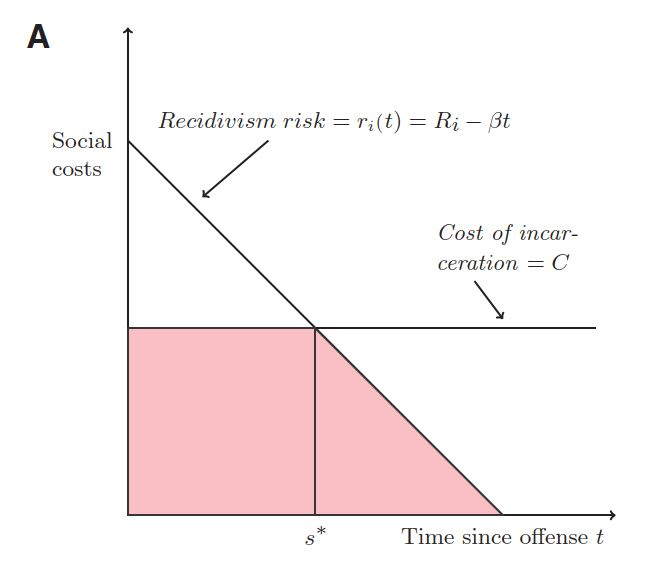
\includegraphics[scale=0.60]{fig1.JPG}
\caption{Total social cost at optimal time-served $s^*$ for a linear recidivism-risk function $r_i(t) = R_i - \beta t$}
\label{fig:Figure 1}
\end{figure}

\begin{figure}[h]
\centering
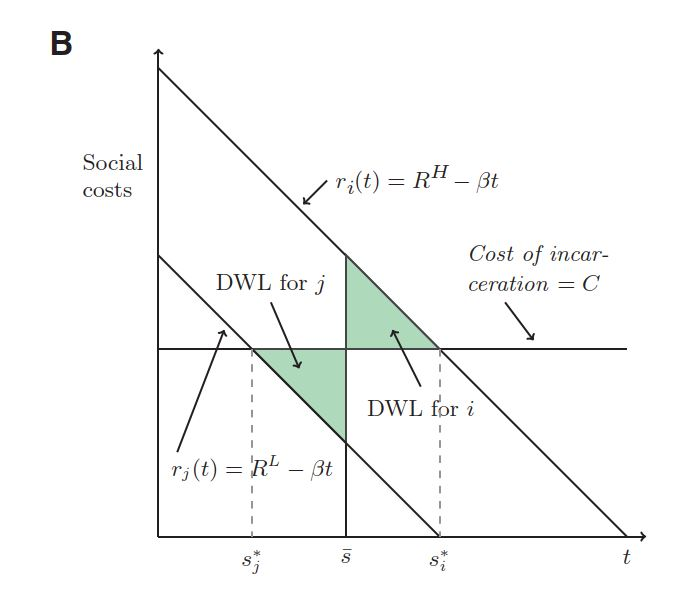
\includegraphics[scale=0.60]{fig2.JPG}
\caption{Dead-weight loss of a fixed release date $s$ relative to optimal $s^*_i$ for a high risk $(R_i = R^{High})$ inmate and optimal $s^*_j$ for low risk $(R_j = R^Low)$}
\label{fig:Figure 2}
\end{figure}





\newpage
\section{Discussion}
\subsection{Welfare}
After several years, it is clear that EM has been almost desperately applied without adequate vision, planning, program integration, staff training, and concurrent research. It has punished, perhaps more humanely and cheaply, and it has been an element in the avoidance of prison crowding and prison construction, but it is not free and it is not without unintended effects. 

In times with large prison populations and discussions regarding downsizing, it is important to recognize that alternative sanctions can have positive influences on young offenders future outcome, both in terms of recidivism and in regards to labor participation \textbf{Andersen 2014} \cite{Andersen2014} and educational outcomes. These findings are important in order to evaluate the returns of introducing noncustodial sanctions and to inform future policy decisions and discussion on electronic monitoring. It will, however, be important to do further qualitative and quantitative research to achieve a deeper understanding of the mechanisms behind these results: \textit{how} the different program elements affect offenders future outcomes, \textit{how} sanction types influence educational trajectories and \textit{how} different outcomes like crime, education and labor market participation are interrelated. 

\newpage
\section{Conclusion}

\newpage
\section{Appendix}


\newpage
\bibliographystyle{plain}
\bibliography{references}
\end{document}
